%%%%%%%%%%%%%%%%%%%%%%%
\section{Internet Network Infrastructure}\label{sec:ISP}
%%%%%%%%%%%%%%%%%%%%%%%

\begin{figure*}
  \begin{center}
  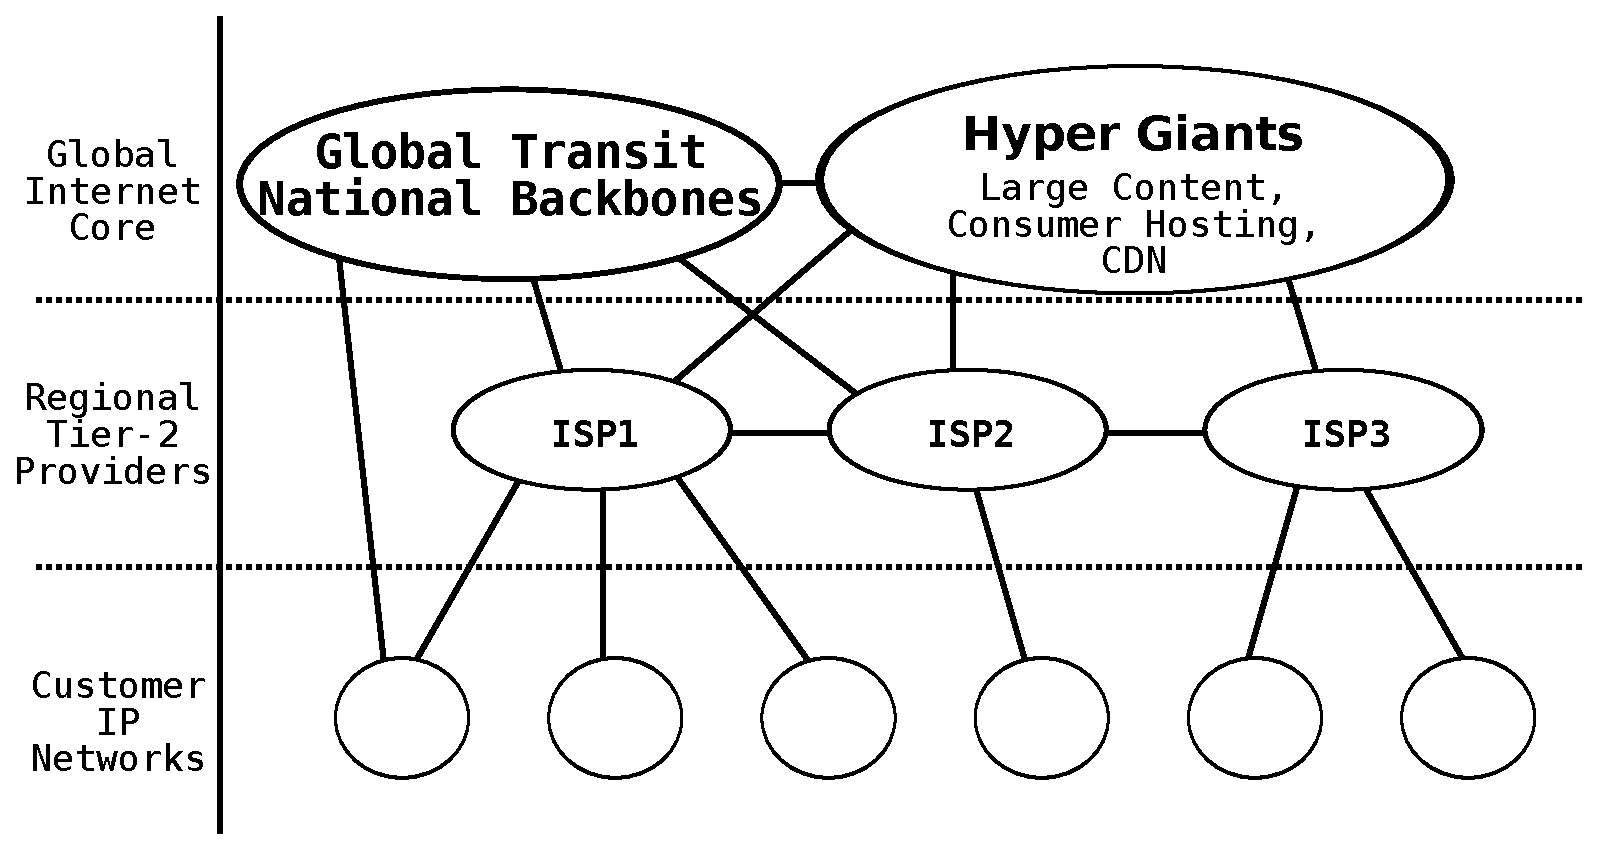
\includegraphics[width=\linewidth]{figures/Internet-Layout.eps}
  \end{center}
  \caption{Layout of the Internet Structure }
  \label{fig:InternetLayout}
\end{figure*}

The Internet Network Infrastructure is provided by a set of Internet Service
Providers (ISPs).  An ISP is, in general terms, an organization that provides
access to the Internet for its customers.  The Internet is structured by the
interconnection of multiple individual networks run by ISPs.  However, control
of an individual network remains solely with the ISP operating it. Figure~\ref
{fig:InternetLayout} shows how the Internet is structured today~\cite{arbor}.
Here, the ISPs run their own networks. This forces a clear distinction between
the individual network that an ISP runs and the global Internet as a network of
networks.  Also, from this, it can be deduced that nobody has control over the
Internet, but instead each ISP has only control over its own network and the
direct connections to other networks.


To be able to interconnect with other networks, an ISP needs to operate an
autonomous system (AS). An AS is an administrating entity, generally under the
control of one administrative domain. On the technical side, each AS is usually
managed by an Interior Gateway Protocol (IGP), \eg OSPF~\cite{RFC2328} or
ISIS~\cite{RFC1142} while the Border Gateway Protocol (BGP~\cite{RFC4271}) is
the de-facto standard for interconnecting different ASes. For more information
and additional details about the Internet topology, we'd like to refer the
reader to Chapter 7 of this book~\cite{ebook-chapter7-Redux}.


\subsection{Traffic Engineering in an AS}

\begin{figure} \begin{center}
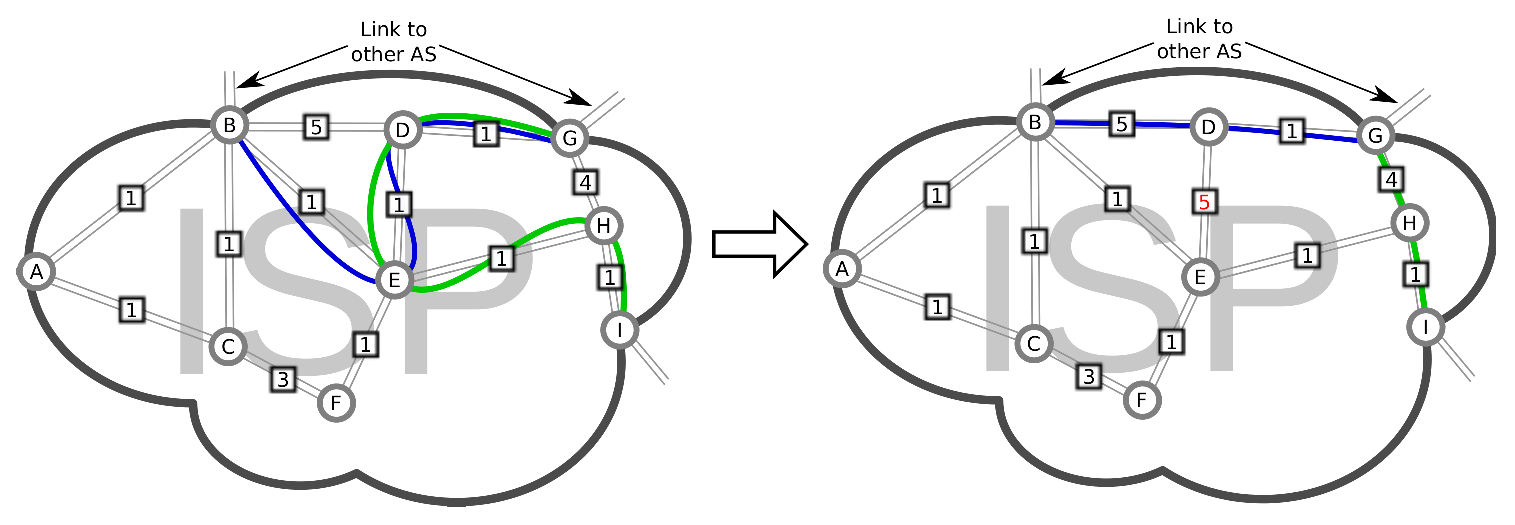
\includegraphics[width=1\linewidth]{figures/Classic-TE.eps} 
\end{center} 
\caption{IGP based Traffic Management Example} 
\label{fig:SimplifiedTE} 
\end{figure}

The greatest challenge for an ISP is to keep its infrastructure operating
efficiently. This is especially hard, since the ISP itself controls neither the
behavior, nor the source nor destination of the majority of the traffic it
carries. The destination of the traffic is determined by the end-users the ISP
sells services to, while the source is usually operated by a Content Delivery
Infrastructure (CDI). The behavior is dictated through end-users requesting
content, and by the operational choices of the CDI. ISPs today tackle the
problem of network operation efficiency by performing Traffic Engineering (TE).
In its broadest sense, today's TE encompasses the application of technology and
scientific principles to the measurement, characterization, modeling, and
control of Internet traffic~\cite{Awduche_OverviewTE:2002}. Today, traffic
engineering reduces to controlling and optimizing the routing function and to
steering traffic on an Origin-Destination (OD) flow basis through the network
in the most effective way.

Traffic Engineering encompasses multiple steps in order to be performed
successfully. First, an ISP needs to record its traffic volume in terms of
Origin-Destination flows. This means keeping traffic statistics of how much
traffic flows from one router in the network to another. Once the OD flows have
been successfully recorded, TE uses this information to simulate the network
behavior with different IGP configurations. The goal of these simulations is to
find an IGP configuration that spreads the network load as evenly as possible.

Figure~\ref{fig:SimplifiedTE} shows an example of how an IGP configuration can
be used to engineer traffic. The labeled circles represent routers, while the
numbers in the squares represent the IGP-weight for the link. For ease of
presentation, the weights for each link are set to the same value for both
directions. An OD flow, which starts at one router and finishes at another,
takes the path through the network that yields the smallest sum over all
weights along the path. For example, in the starting configuration of the
network (Figure~\ref {fig:SimplifiedTE} (left)) the flow $IG$ does not take the
direct path $I \rightarrow H \rightarrow G$ two, since according to the IGP
weights, a more effective path exists. In fact, the path $I \rightarrow H
\rightarrow E \rightarrow D \rightarrow \ G$ has an accumulated weight of 4
instead of 5 (green path). All traffic at router I destined for router G takes
this path. Similarly, all traffic that originates from B and goes to G follows
the path $B \rightarrow E \rightarrow D \rightarrow G$ (blue path). Also, both
paths share links, leading to a possible overload situation. In order to solve
this problem, we choose to modify the link weight between the routers D and E.
By increasing the weight from 1 to 5 (marked red in the right network), the
blue as well as the green paths are shifted to the direct path. The change is
shown in Figure~\ref{fig:SimplifiedTE} (right).

This simple diagram allows for illustrating multiple caveats that IGP based
traffic engineering introduces. First, IGP-based traffic engineering affects
traffic on an OD-flow basis only. This means that the path from one router to
another can be changed, but the traffic on the OD flow cannot be split onto
multiple paths. Secondly, the change of one weight can affect multiple OD-flows
at the same time. Thus, the weights have to be changed very carefully. In the
worst case, it might not be possible to fully separate some OD-flows due to the
network layout.

One caveat is not immediately obvious but needs to be taken into account when
performing traffic engineering. While the link weights are usually known to all
routers, they are propagated by messages that routers exchange. This
propagation takes time, which can lead to short-term inconsistencies in the
view of a network. We again use Figure~ \ref{fig:SimplifiedTE} for illustrating
this. When the link weight is changed as described in the example explained
before, routers D and E update their routing. This has an immediate effect on
the traffic from B to G. With the update, the shortest path from router E to G
is now $E \rightarrow H \rightarrow G$. In accordance, E configures its routing
to send all traffic for G through H. However, H has not converged at this point
and still uses the old path ($H \rightarrow E \rightarrow D \rightarrow G$).
Thus, H still sends all traffic for G towards E. As long as H uses the outdated
IGP weight information, all traffic for G that reaches either E or H is sent
back and forth between the two routers. This forwarding, on the one hand,
likely overloads the link. On the other hand, most traffic that is affected by
this will be dropped due to its time-to-live (TTL) running out.

The work of Francois \etal~\cite{transient-IGP} shows that it is possible to
gradually change IGP weights by sequentially ordering changes. Accordingly,
routing loops like those in the example are avoided. However, these changes
still require time during which the network can be in a transient state with
overloaded links. Besides the challenges induced by optimizing the IGP, this
approach also assumes that traffic is predictable and stable over time. By
running simulations based on past traffic aggregates to engineer the routing
for the future, it is implicitly assumed that traffic patterns remain similar
over a longer period of time.

With the emergence of CDIs, however, traffic has become volatile in terms of
its origin. In fact, CDIs can shift massive amounts of traffic in a matter of
seconds from one server cluster to another. While this behavior is needed and
propagated by CDIs to cope with volatile demand surges, it is in stark contrast
to the ISP's traffic engineering, which assumes traffic behavior to be stable
for days, weeks or sometimes months.


%%%%%%%%%%%%%%%%%%%%%%%
\subsection{Domain Name System Basics}\label{sec:DNS}
%%%%%%%%%%%%%%%%%%%%%%%

\begin{figure}[tbp] \begin{center}
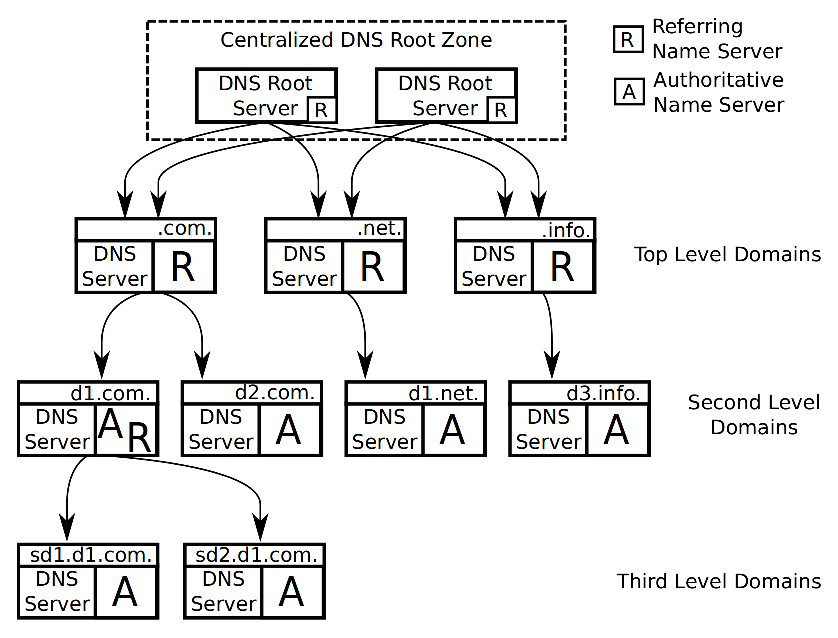
\includegraphics[width=0.8\linewidth]{figures/DNSHierarchy.eps} 
\end{center}
\caption{Example DNS hierarchy} 
\label{fig:DNS-Hierarchy} 
\end{figure}

The Domain Name System (DNS) plays a major role in today's Internet
architecture and is an essential component of any Web based content delivery
architecture.  DNS relies on a distributed database with a hierarchical
structure. The root zone of the DNS system is centrally administered and serves
its {\em zone} information via a collection of {\em root servers}.  The root
servers delegate responsibility for specific parts (zones) of the hierarchy to
other {\em name servers}, which may in turn delegate the responsibility to
other name servers.  At the end, each site is responsible for its own {\em
domain} and maintains its own database containing its information and operates
an {\em authoritative} name server.

The whole DNS database is usually queried by end-hosts using a local name
server called {\em caching resolver}. If this name server receives a query for
a domain that it does not know about, it fetches this information from another
name server. If the server does not know how to contact the authoritative
server for a zone, it will query a root server\footnote{The first query can go
to some authoritative server below the root if there exists cached
information.}. The root server will \emph{refer} the resolver to another server
that is authoritative for the domain that is immediately below the root and of
which the zone is a part. The resolver will then query this server, and so
forth, stepping down the tree from the root to the desired zone.

To illustrate this process, Figure~\ref{fig:DNS-Hierarchy} show a sample DNS
hierarchy. In this case, the root of the DNS name space, denoted with a '.', is
hosted on two \emph{DNS root servers}. Both servers are under one
administrative control, and both can refer a request to any of the top level
domain servers. Here, three domains exist, \ie \textit{.com}, \textit {.net}
and \textit{.info}. Again, these name servers refer to the second level
domains. Since the domain name are concatenated together as the hierarchy is
traversed, the domains that are now possible are \textit {d1.com.}, \textit
{d2.com.}, \textit{d1.net.} and \textit{d3.info.}. At this point, the second
level domains d1.net. and d3.info have reached their authoritative resolver.
For example, a query to the name server of \textit{.d3} for
\textit{www.d3.info} is answered authoritatively from there. Note that the name
servers for the second level domains are operated by independent entities that
know nothing of each other. Thus, the database is distributed, while each party
is responsible for its own zone.  Finally, the name server of \textit{.d1.com.}
has a dual role. While it is referring the subdomains \textit{.sd1.d1.com.} and
\textit{.sd2.d1.com.} to other name servers, it also answers queries for other
names in its name space authoritatively.  This means that a query for
\textit{www.d1.com.} is directly answered, while a query for
\textit{www.sd1.d1.com} is referred to the name server responsible for
\textit{.sd1.d1.com}.

For efficiency reasons DNS relies heavily on caching
\cite{DNS-caching,DNS-IMC-2010}. All information that a name server delivers to
a resolver is cached for a duration specified in the time-to-live (TTL) field
of the {\em resource records} (RR). Caching today is usually also performed on
end-hosts by the operating system's {\em stub resolver}, as well as
applications, \eg web browsers.

\noindent\textbf{DNS Today.}\label{section:dns-today} When DNS was introduced in
1983, its sole purpose was to resolve host names into IP addresses in a more
scalable fashion than the until then used \texttt{hosts} file. Since then a
number of features and new uses have found their way into the now omnipresent
DNS. In addition to the increasing complexity within the DNS protocol itself
\cite {DNSComplexity2007}, new and oftentimes unforeseen (ab)uses have been
established. Paul Vixie gives an overview in \cite{WhatDNSIsNOT2009}. The most
important points of critique are as follows:

\begin{description} \item[CDI load balancing:] Content delivery infrastructures
set short TTLs on their DNS answers to allow for short reaction times to
shifting loads. Short TTLs impede on cacheability and therefore increase the
load on the whole DNS system. In addition, CDIs tailor their reply for the IP
address of the requesting resolver using the assumption that the DNS resolver
is close to the client originating the request. It has been shown in the past
that this assumption is quite often wrong~\cite
{Precise:Mao2002,dns-redirection,DNS-IMC-2010,DNS-extension-IP-client}.

\item[NXDOMAIN catcher:] Some ISPs and third party DNS providers mangle a
negative reply with the NXDOMAIN status code into a positive one with the IP
address of a search website under the control of the ISP. By hosting
advertisements along the search results it is easily possible to increase the
profit margin. While this may work to some degree for web browsing,
applications relying on proper delivery of NXDOMAIN records, \eg email, are
inevitably hampered.  \end{description}

A third-party ecosystem around DNS has evolved over the last couple of years.
Players like OpenDNS, AdvantageDNS, UltraDNS, and most recently Google offer
open resolvers to anyone with different feature sets. OpenDNS Basic does
NXDOMAIN catching but offers phishing and botnet protection for free.
Furthermore, OpenDNS increases the service level for payment between 5 dollars
a month up to several thousand dollars per year for business customers. When
Google Public DNS entered the market, their highest-valued goals were to
``speed up your browsing experience'' and to ``improve your security''. To
achieve both targets Google advertises an impressive list of optimizations and
fine tuning~\cite{googledns}, \eg prefetching, load balancing with shared
cache, validity checking, and nonce prepending. Google Public DNS also refrains
from utilizing NXDOMAIN to make profit. From an implementation perspective,
most if not all of the third-party resolvers host their DNS servers on multiple
sites around the globe and use anycast to guide DNS clients to the nearest
resolver.

In this open market space a user annoyed by his ISP's DNS can easily choose for
cost-free third-party service.  Tools such as namebench~\cite{namebench} might
help him in choosing a well-performing one. The irony however is that a user,
by choosing a different DNS than the one assigned by his ISP, will most likely
undermine the traffic matrix optimizations performed by CDIs and ISPs, and can
potentially even lower his quality of experience due to longer download
times~\cite{DNS-IMC-2010}.
